
\begin{figure*}
    \centering
    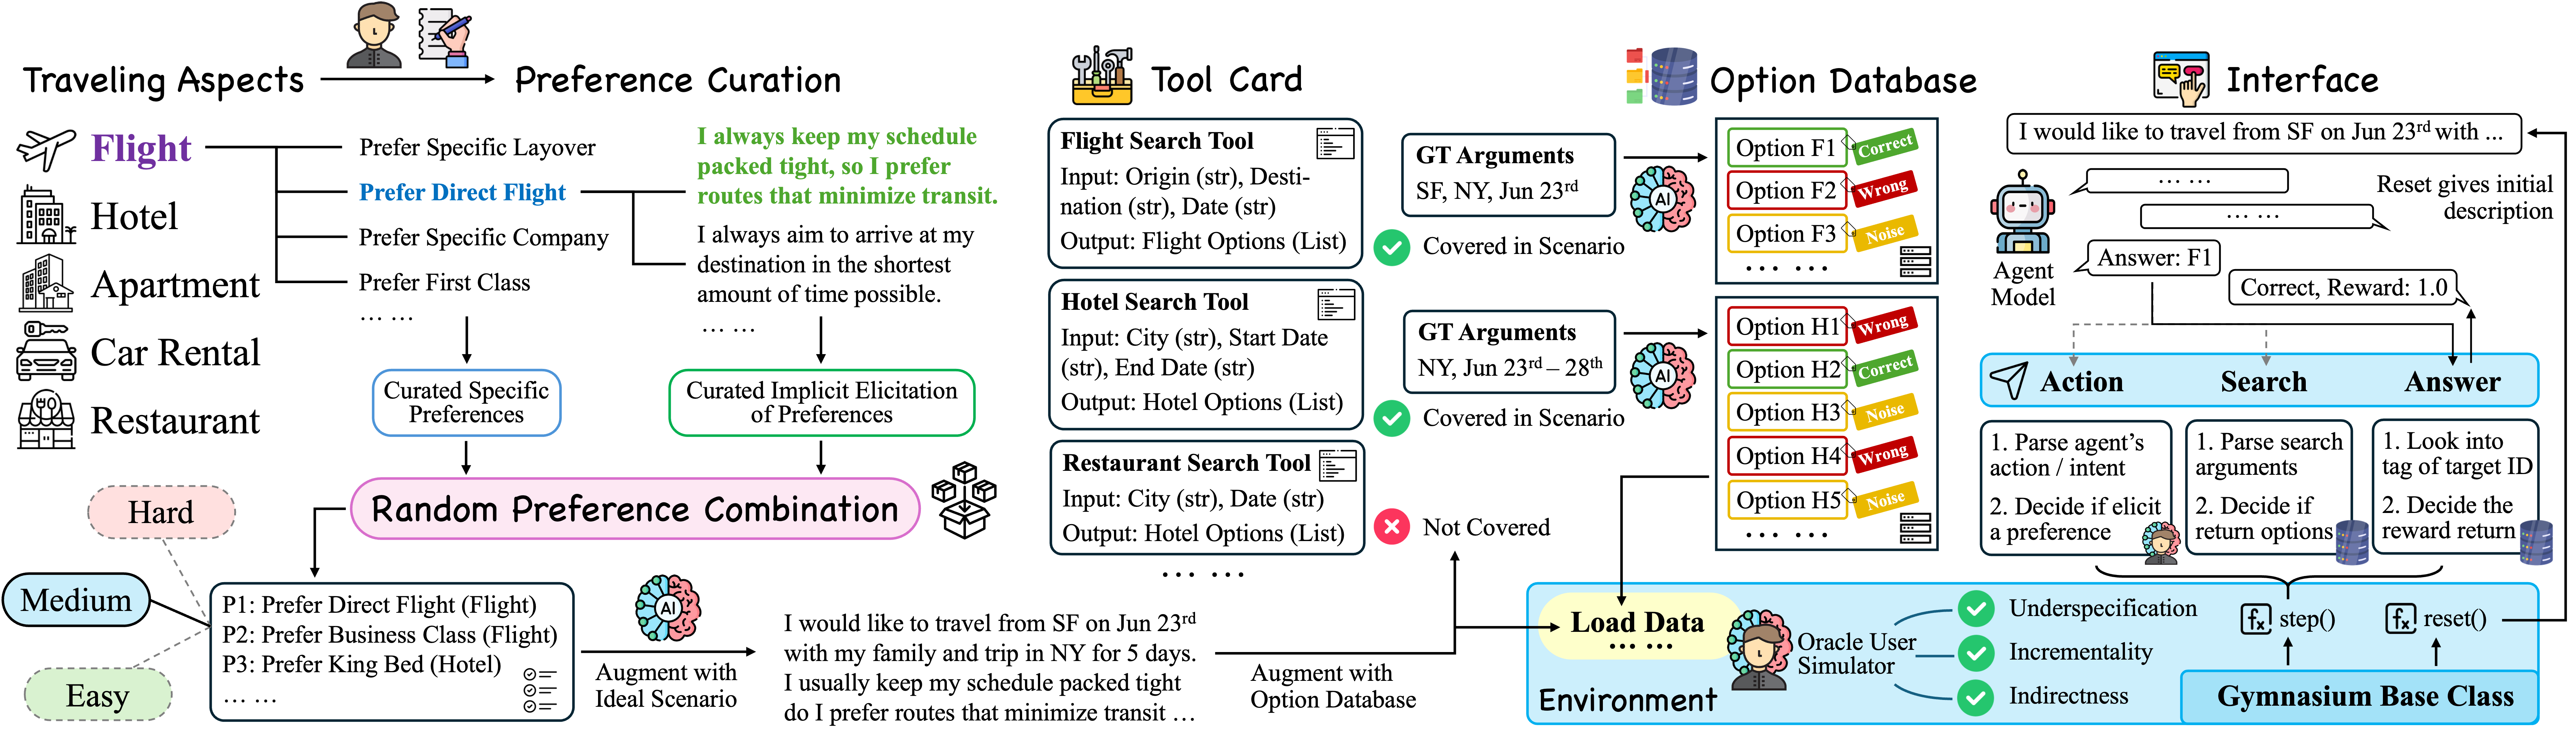
\includegraphics[width=\linewidth]{figures/pipeline.png}
    \caption{The pipeline of {\gymname} Construction, including data gathering, preference curation, tool augmentation, environment setup and interface design. \textit{Random Preference Combinations} makes our pipeline highly scalable and enables the efficient generation of even 10K+ data points.} 
    \label{fig:pipeline}
\end{figure*}


\section{{\gymname}}

We build {\gymname} upon the standardized gymnasium environment, focusing on travel planning tasks where users gradually reveal their preferences in implicit ways. Compared to prior work, {\gymname} features a significantly more diverse and grounded collection of user preferences, each paired with carefully curated implicit expressions, and supports tool-augmented search with injected noise and cost-awareness. This setting challenges agents to perform search and reasoning in a user-centric manner, under constraints of partial, evolving, and indirect preference information. We describe the gym design details in the following.

\subsection{Data Gathering}

As shown in \Cref{fig:pipeline}, we begin by identifying five core aspects of travel planning: flight, hotel, apartment, car rental, and restaurant. Our data gathering is guided by three key principles: \textit{realism}, \textit{diversity}, and \textit{implicitness}. First, we ensure realism by curating preferences that reflect plausible, real-world user needs—such as preferring direct flights (flight) or king-sized beds (hotel). Second, we aim for diversity by collecting around a hundred distinct preferences that span travel aspects. Third, we emphasize implicitness by pairing each preference with multiple naturally phrased statements that express the intent indirectly. For instance, the preference for direct flights might be expressed as: ``I always keep my schedule packed tight, so I prefer travel routes that minimize transit time.'' These implicit expressions are carefully curated and validated to ensure that (i) they do not reveal the preference explicitly, and (ii) they still clearly imply the intended preference without ambiguity.

These curated preferences and their associated implicit expressions serve as the foundation for generating travel scenarios. We randomly sample and combine preferences across the five aspects, categorizing the resulting data into three difficulty tiers based on the number of preferences involved. For each combination, we generate an ideal travel arrangement statement that incorporates all relevant preferences using GPT-4o. This finally forms a data point in our environment.

\subsection{Tool Augmentation}
For each travel planning aspect, we develop a corresponding tool that simulates a database search. For example, the flight search tool accepts origin, destination, and date, returning a list of mock options. Instead of querying real-time data, we rely on pre-generated options to ensure stable and controlled tool outputs. This design choice is justified because (i) it guarantees consistency and quality of returned results, and (ii) our focus is user-centric reasoning rather than challenges of online search.

Each data point is associated with a tailored database of options for all relevant travel planning aspects. Specifically, for each aspect, we generate three types of options: correct (satisfying all preferences), wrong (violating at least one preference), and noise (incomplete or irrelevant to the query, such as a flight option with a destination different from the one the user searched for). These options are mixed to form the complete search space, with each data point containing up to over 100 options. Option generation is handled by GPT-4o under human supervision to ensure quality and diversity.

\subsection{Environment Building}
Each data point in the environment contains a travel scenario, a set of implicit user preferences, and a database of relevant options. The environment simulates an oracle user with access to these internal states, while engaging in multi-turn interactions with a agent model under test. Upon reset, the environment provides only basic trip information and high-level requirements (e.g., hotel or flight), without disclosing any of its specific preferences. Preferences are then elicited over time, either (i) when the tested model explicitly asks about a relevant aspect, or (ii) after a fixed number of turns without progress (see \Cref{sec:apdx_construction} for details), at which point a preference is randomly and proactively revealed. All elicited preferences are presented implicitly, in line with the associated data.

This design captures the three key traits and challenges we previously identify: \textit{underspecification}, where only coarse needs are initially provided; \textit{incrementality}, where user preferences emerge progressively as the conversation evolves; and \textit{indirectness}, where preferences are stated implicitly through natural, carefully-curated, heuristic-based language. These properties reflect real-world user behaviors and make {\gymname} a robust testbed for user-centric reasoning.

\subsection{Agent Interaction}
We provide a standardized interaction interface for agents, supporting three types of actions: \texttt{action}, \texttt{search}, and \texttt{answer}. Through \texttt{search}, agents issue queries specifying the travel planning aspect and arguments (e.g., hotel with specific dates), which are matched against ground truth. If the arguments match, the environment returns the mixed set of relevant options; otherwise, it returns nothing. Through \texttt{action}, the agent communicates with the user, typically by asking clarifying questions. The environment interprets the intent and responds naturally, potentially revealing a preference in an implicit form. Finally, through \texttt{answer}, the agent selects its recommended option ID(s), which are evaluated against the ground-truth correct options. Since ideal itineraries often span multiple aspects, correct answers may include several options.

\begin{table*}[!t]
\begin{center}
\small
\tabcolsep=0.015\linewidth
\resizebox{\linewidth}{!}{
\begin{tabular}{lccll|lll|lcc}
\toprule
\textbf{Difficulty Tier} & \textbf{\# Test} & \textbf{\# Train} & \textbf{Composition} & & \multicolumn{2}{c}{\textbf{Global Dataset Metadata}} & & \textbf{Travel Aspect} & \textbf{\# Scenarios} & \textbf{Preferences} \\
\midrule
Easy   & 118 & 666 & Travel-22, 2222   & & Travel Aspects       & 5   &                         & Hotel       & 187 (39.7\%) & 15 \\
Medium & 201 & 1130 & Travel-33, 233, 333   & & Pref. Categories     & 24  &                         & Restaurant  & 298 (63.3\%) & 19 \\
Hard   & 152 & 855 & Travel-44, 334, 444 & & Total Prefs.         & 82  &                         & Flight      & 275 (58.4\%) & 16 \\
\multicolumn{4}{l}{-----------------------------------------------------------------------------} & & Elicitation Ways     & 902 &                         & Rental Car  & 243 (51.6\%) & 14 \\
\textbf{Total} & \textbf{471} & 2651 & \textbf{{\gymname} Test} / Train &  & Options (B/C/W/N)     & 1/3/10/5 &                   & Apartment    & 172 (36.5\%) & 18 \\
\bottomrule
\end{tabular}
}
\end{center}
\vspace{-3mm}
\caption{\textbf{{\gymname} Statistics:} Difficulty-tiered statistics (left), global configuration metadata (middle), and travel aspect coverage (right). \textit{Pref.} denotes preference; \textit{B/C/W/N} stands for Best, Correct, Wrong, and Noise options respectively; \textit{\# Scenarios} indicates the number of data scenarios in which each travel aspect appears.}
\label{tab:statistics}
\end{table*}


\subsection{Variants, Scalability and Statistics}
\label{sec:variants}
{\gymname} supports several extensions. First, it can simulate a noisy search environment where query results are corrupted at a configurable frequency, mimicking real-world web or tool errors. Second, it allows for budget-aware decision-making by rewarding models that not only find correct options but also select the most cost-effective ones (best option). A hyperparameter can control the strength of this reward, encouraging agents to optimize toward practical utility.

As illustrated in \Cref{fig:pipeline}, the Random Preference Combination strategy enhances both the diversity and scalability of our data construction, enabling over 10K distinct scenarios. To manage computational costs during benchmarking, we use 417 data points for testing and reserve 2651 for training, which are not used in benchmarking but may support future model training (see Discussion section). Detailed statistics of {\gymname} are presented in \Cref{tab:statistics}. For instance, ``Travel-223'' denotes a scenario with three travel aspects: two containing two implicit preferences each, and one with three. Additional details on data and environment construction are provided in the \Cref{sec:apdx_construction}.
